\chapter{Inclined planes}
Take a look at this box resting on an incline plane due to static friction and gravity.

\begin{figure}[htbp] \centering \caption{A box on an inclined plane with $a=0$ due to static friction and gravity.} \begin{tikzpicture}[scale=1, line cap=round, line join=round]  
    \coordinate (A) at (0,0); 
    \coordinate (B) at (5,0); 
    \coordinate (C) at (5,2); 
    % sets the approximate slope of the hypotenuse 
    % triangle 
    \draw (A)--(B)--(C)--cycle; 
    \draw[->] (0,0) -- (0,2) node[left] {$y$}; 
    \draw[->] (0,0) -- (5,0) node[below] {$x$}; 
    \draw (A) ++(0:0.8) arc (0:22:0.8); 
    \node at ($(A)+(1.05,0.25)$) {$\theta$};
    \path (A) -- (C) coordinate[pos=0.5] (M); 
    \draw[shift={(M)},rotate=22, yshift=0.31cm] (-0.3,-0.3) rectangle (0.3,0.3); 
    \coordinate (O) at (6,2); \draw[->, thick] (O) -- ++(1,0) node[below right] {$x$}; 
    \draw[->, thick] (O) -- ++(0,1) node[left] {$y$}; 
\end{tikzpicture}
 \label{fig:example} 
\end{figure} 

Now for objects on an incline, such as a box on a ramp, we will want to tip our coordinate system. Why you ask? Because we are not restricted to having our y-axis 90$^\circ$ vertically and our x-axis flat horizontally. In this case we can tip our axes so that the x-axis is parallel to the incline and the y-axis is perpendicular to the incline, aligning with the normal force. This will make our calculations much easier.
\begin{figure}[htbp]
    \centering

    \begin{subfigure}{0.4\textwidth}
        \centering
        \begin{tikzpicture}[scale=0.55]
            \draw[->, thick] (0,0) -- (0,-5) node[below] {$F_g$};        
            \draw[->, thick] (0,0) -- (3, 2) node[above right] {$F_F$};        
            \draw[->, thick] (0,0) -- (-2, 4) node[left] {$F_N$};    
            \draw[->, dashed, thin] (0,0) -- (5, 0) node[right] {$x$};

            \draw (0,0) ++(0:2) arc (0:33:2); 
            \node at ($(0,0)+(1.05,0.3)$) {$\theta$};

            \draw[->, thick] (4,4) -- ++(2,0) node[below right] {$x$};
            \draw[->, thick] (4,4) -- ++(0,2) node[left] {$y$};
            \filldraw[fill=red, draw=red] (0,0) circle [radius=0.25cm];
        \end{tikzpicture}
        \caption{Free body diagram in standard orientation.}
        \label{fig:fbd-standard}
    \end{subfigure}
    \hfill
    \begin{subfigure}{0.4\textwidth}
        \centering
        \begin{tikzpicture}[scale=0.55]
            \begin{scope}[rotate=-22]
                \draw[->, thick] (0,0) -- (0,-5.2) node[below left] {$F_g$};        
            \end{scope}
            \begin{scope}[rotate around={-22:(4,4)}]
                \draw[->, thick] (4,4) -- ++(2,0) node[below right] {$x$};
                \draw[->, thick] (4,4) -- ++(0,2) node[left] {$y$};
            \end{scope}
            \draw[->, thick] (0,0) -- (3, 0) node[above right] {$F_F$};        
            \draw[->, thick] (0,0) -- (0, 4) node[left] {$F_N$};    
            \draw[thin, dashed] (0,0) -- (0, -5) node[right] {$F_{gy}$};    

            % \def\theta{22}
            % Draw small angle θ between F_g (tilted) and vertical F_gy, on correct side
            \draw[thin] (0,-2) arc (-90:-90-22:2);
            \node at ({-0.8*sin(22/2)},{-0.8*cos(22/2)}) [below] {$\theta$};

            \draw[->, thin, dashed] (0,-5) -- (-{5*sin(22)},-5) node[below right] {$F_{gx}$};
            \filldraw[fill=red, draw=red] (0,0) circle [radius=0.25cm];

        \end{tikzpicture}
        \caption{Axes rotated by $\theta$.}
        \label{fig:fbd-rotated}
    \end{subfigure}
    \caption{Free body diagrams on an incline.}
    \label{fig:fbd-both}
\end{figure}

From this new perspective, we can see that the gravitational force $F_g$ can be broken down into two components: one parallel to the incline ($F_{gx}$)\footnote{Note that some professors will use down the incline as positive. This book will consistently use up the incline as positive as rotating coordinate plane aligns well with this.} and one perpendicular to the incline ($F_{gy}$). The normal force $F_N$ acts perpendicular to the surface of the incline, while the frictional force $F_F$ acts parallel to the surface, opposing motion. The coordinate planes in the corner are included to show the original coordinate system relative to our rotated FBD.\footnote{Note also that the dashed line components are not actual forces, they are drawn in for illustration of how forces at angles effect the standard forces.}
  
We can set up the following equations based on Newton's second law:

$$\sum F_x = F_{gx} - F_F = m a_x = 0,\qquad \sum F_y = F_N - F_{gy} = m a_y = 0$$

Using the trigonometric components, we can express the forces in terms of the angle $\theta$:

$$\sum F_x = mg\sin(\theta) - F_F = m a_x = 0,\qquad \sum F_y = F_N - mg\cos(\theta) = m a_y = 0$$

Solving for the normal force and frictional force, we find:
$$F_N = mg\cos(\theta),\qquad F_F = mg\sin(\theta)$$

The following relationships are true for acceleration on an incline:
$$F_F = \mu F_N, \qquad a_x = g(\sin\theta - \mu \cos\theta)$$
Where $\mu$ is the coefficient of friction between the box and the incline.

Let's apply all of this to an example problem:
\begin{Exercise}[title=Box sliding down an incline, label=incline1]
    A 30 kg block is sliding down an incline plane that makes a $30^\circ$ with the horizontal. Given that the coefficient of kinetic friction is 0.3, find the following. Note that up the inclined plane is considered the positive x-direction.
    \begin{enumerate}[label=(\alph*)]
        \item The normal force acting on the block.
        \item The frictional force acting on the block.
        \item The acceleration of the block down the incline.
    \end{enumerate}

\begin{center}
    

% Gradient Info
  
\tikzset {_oxpa7yony/.code = {\pgfsetadditionalshadetransform{ \pgftransformshift{\pgfpoint{0 bp } { 0 bp }  }  \pgftransformrotate{0 }  \pgftransformscale{2 }  }}}
\pgfdeclarehorizontalshading{_b0fvkm42y}{150bp}{rgb(0bp)=(0.65,0.81,0.87);
rgb(37.5bp)=(0.65,0.81,0.87);
rgb(62.5bp)=(0.14,0.33,0.54);
rgb(100bp)=(0.14,0.33,0.54)}
\tikzset{every picture/.style={line width=0.75pt}} %set default line width to 0.75pt        

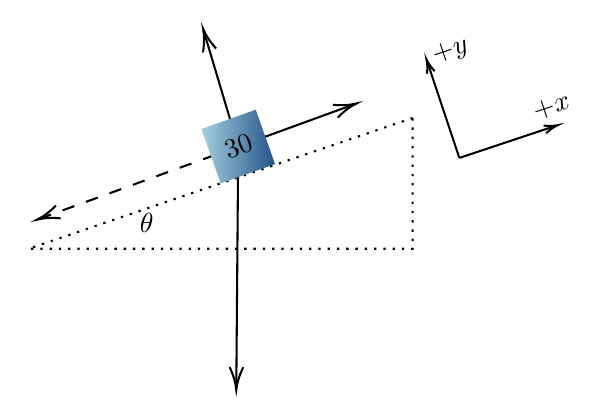
\begin{tikzpicture}[x=0.75pt,y=0.75pt,yscale=-1,xscale=1]
%uncomment if require: \path (0,300); %set diagram left start at 0, and has height of 300

%Straight Lines [id:da6260155651515338] 
\draw  [dash pattern={on 4.5pt off 4.5pt}]  (126.94,59.76) -- (31.88,94.32) ;
\draw [shift={(30,95)}, rotate = 340.02] [color={rgb, 255:red, 0; green, 0; blue, 0 }  ][line width=0.75]    (10.93,-3.29) .. controls (6.95,-1.4) and (3.31,-0.3) .. (0,0) .. controls (3.31,0.3) and (6.95,1.4) .. (10.93,3.29)   ;
%Straight Lines [id:da07021534869254287] 
\draw    (126.94,59.76) -- (110.57,4.92) ;
\draw [shift={(110,3)}, rotate = 73.38] [color={rgb, 255:red, 0; green, 0; blue, 0 }  ][line width=0.75]    (10.93,-3.29) .. controls (6.95,-1.4) and (3.31,-0.3) .. (0,0) .. controls (3.31,0.3) and (6.95,1.4) .. (10.93,3.29)   ;
%Straight Lines [id:da0033380673706231434] 
\draw    (126.94,59.76) -- (182.12,39.68) ;
\draw [shift={(184,39)}, rotate = 160.01] [color={rgb, 255:red, 0; green, 0; blue, 0 }  ][line width=0.75]    (10.93,-3.29) .. controls (6.95,-1.4) and (3.31,-0.3) .. (0,0) .. controls (3.31,0.3) and (6.95,1.4) .. (10.93,3.29)   ;
%Straight Lines [id:da23520098564851555] 
\draw    (126.94,59.76) -- (126.02,175) ;
\draw [shift={(126,177)}, rotate = 270.46] [color={rgb, 255:red, 0; green, 0; blue, 0 }  ][line width=0.75]    (10.93,-3.29) .. controls (6.95,-1.4) and (3.31,-0.3) .. (0,0) .. controls (3.31,0.3) and (6.95,1.4) .. (10.93,3.29)   ;
%Shape: Right Triangle [id:dp466382574170195] 
\draw  [dash pattern={on 0.84pt off 2.51pt}] (211,46) -- (26,109) -- (211,109) -- cycle ;
%Shape: Square [id:dp4389428644687856] 
\draw  [draw opacity=0][shading=_b0fvkm42y,_oxpa7yony] (109.2,51.32) -- (135.38,42.02) -- (144.68,68.2) -- (118.5,77.5) -- cycle ;
%Straight Lines [id:da8405281832946017] 
\draw    (233.47,65.25) -- (279.01,50.09) ;
\draw [shift={(280.9,49.45)}, rotate = 161.58] [color={rgb, 255:red, 0; green, 0; blue, 0 }  ][line width=0.75]    (6.56,-1.97) .. controls (4.17,-0.84) and (1.99,-0.18) .. (0,0) .. controls (1.99,0.18) and (4.17,0.84) .. (6.56,1.97)   ;
%Straight Lines [id:da9798112871779567] 
\draw    (218.3,19.71) -- (233.47,65.25) ;
\draw [shift={(217.67,17.82)}, rotate = 71.58] [color={rgb, 255:red, 0; green, 0; blue, 0 }  ][line width=0.75]    (6.56,-1.97) .. controls (4.17,-0.84) and (1.99,-0.18) .. (0,0) .. controls (1.99,0.18) and (4.17,0.84) .. (6.56,1.97)   ;

% Text Node
\draw (78,90.4) node [anchor=north west][inner sep=0.75pt]    {$\theta $};
% Text Node
\draw (126.94,59.76) node  [rotate=-340]  {$30$};
% Text Node
\draw (279.83,46.23) node [anchor=south] [inner sep=0.75pt]  [rotate=-341.58]  {$+x$};
% Text Node
\draw (219.56,17.18) node [anchor=west] [inner sep=0.75pt]  [rotate=-341.58]  {$+y$};


\end{tikzpicture}
\end{center}
    
\end{Exercise}
\begin{Answer}[ref=incline1]
    \begin{enumerate}[label=(\alph*)]
        \item The normal force must be equal to the perpendicular component of the gravitational force, since there is no acceleration in the y-direction of our rotated y-axis:
        $$F_N = mg\cos(\theta) = (30\,\text{kg})(9.8\,\text{m/s}^2)\cos(30^\circ) \approx 254.6\,\text{N}$$
        \item The frictional force can be found using the coefficient of kinetic friction and the normal force:
        $$F_F = \mu_k F_N = (0.3)(254.6\,\text{N}) \approx 76.4\,\text{N}$$
        \item The acceleration can be found by setting up the equation for the sum of forces in the x-direction:
        $$\sum F_x = F_F - mg\sin(\theta)  = ma_x$$
        Solving for $a_x$:
        \begin{align*}
            a_x &= \frac{F_F - mg\sin(\theta)}{m} \\
            &= \frac{76.4\,\text{N} - (30\,\text{kg})(9.8\,\text{m/s}^2)\sin(30^\circ) - }{30\,\text{kg}} \\
            &= \frac{76.4 - 147}{30} \\
            &\approx \frac{-70.6}{30} \\
            &\approx -2.35\,\text{m/s}^2 
        \end{align*}
    \end{enumerate}
\end{Answer}

\begin{Exercise}[title=Solving for angle $\theta$, label=incline2]
    A 40 kg box is sitting on a rough inclined plane, held in place by static friction. The coefficient of static friction $\mu_s$ between the box and the incline is found to be 0.464. What is the maximum angle $\theta$ that the incline can be tilted to before the box starts to slide down?
\end{Exercise}
\begin{Answer}[ref=incline2]
For a box to be on the verge of sliding, the frictional force (static) must equal the component of gravitational force parallel to the incline. Thus, we can set up the following equation:
\begin{align*}
    \sum F_x &= mg\sin(\theta) - F_F = 0 \\
    mg\sin(\theta) &= F_F \\
    mg\sin(\theta) &= \mu_s F_N \\
    mg\sin(\theta) &= \mu_s mg\cos(\theta) \\
    \tan(\theta) &= \mu_s \\
\end{align*}

Solving for $\theta$, we get $\theta = \tan^{-1}(\mu_s)$. 
Plugging in the value of $\mu_s$, we get $\theta = 24.89^\circ$
\end{Answer}

\begin{Exercise}[label=incline3, title=Pulleys and Inclines]
    A block at rest of mass $m_1$ is resting on a rough inclined plane making an angle $\theta$ with the horizontal. The coefficient of kinetic friction between the block and the incline is $\mu_k$. The block is attached by a light string over a frictionless pulley to a hanging block of mass $m_2$. Once they are connected by a string, the hanging block begins to descend and the block of $m_1$ moves upwards along the incline. Draw the free body diagrams of each mass. Derive an equation for the acceleration of $m_2$, only in terms of $m_1, m_2, g, \theta, \text{ and } \mu_k$.

    
%Diagram made using mathcha
% Gradient Info
  
\tikzset {_7m272izdc/.code = {\pgfsetadditionalshadetransform{ \pgftransformshift{\pgfpoint{0 bp } { 0 bp }  }  \pgftransformrotate{0 }  \pgftransformscale{2 }  }}}
\pgfdeclarehorizontalshading{_92yru611t}{150bp}{rgb(0bp)=(0.65,0.81,0.87);
rgb(37.5bp)=(0.65,0.81,0.87);
rgb(62.5bp)=(0.14,0.33,0.54);
rgb(100bp)=(0.14,0.33,0.54)}

% Gradient Info
  
\tikzset {_0e7bbdflb/.code = {\pgfsetadditionalshadetransform{ \pgftransformshift{\pgfpoint{89.1 bp } { -128.7 bp }  }  \pgftransformscale{1.32 }  }}}
\pgfdeclareradialshading{_zq02cgox8}{\pgfpoint{-72bp}{104bp}}{rgb(0bp)=(1,1,1);
rgb(0bp)=(1,1,1);
rgb(25bp)=(0.48,0.15,0.15);
rgb(400bp)=(0.48,0.15,0.15)}

% Gradient Info
  
\tikzset {_e13qiwxhl/.code = {\pgfsetadditionalshadetransform{ \pgftransformshift{\pgfpoint{89.1 bp } { -128.7 bp }  }  \pgftransformscale{1.32 }  }}}
\pgfdeclareradialshading{_pf7lzm7ry}{\pgfpoint{-72bp}{104bp}}{rgb(0bp)=(1,1,1);
rgb(0bp)=(1,1,1);
rgb(25bp)=(0.72,0.91,0.53);
rgb(400bp)=(0.72,0.91,0.53)}
\tikzset{every picture/.style={line width=0.75pt}} %set default line width to 0.75pt        

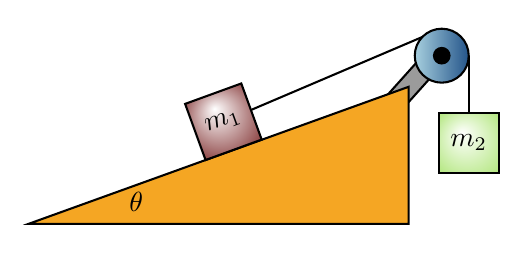
\begin{tikzpicture}[x=0.75pt,y=0.75pt,yscale=-1,xscale=1]
%uncomment if require: \path (0,300); %set diagram left start at 0, and has height of 300

%Straight Lines [id:da7475228986806758] 
\draw    (96.81,53.82) -- (202,9) ;
%Shape: Rectangle [id:dp9330889732935973] 
\draw  [fill={rgb, 255:red, 155; green, 155; blue, 155 }  ,fill opacity=1 ] (191.78,23.14) -- (199.14,29.74) -- (180.22,50.86) -- (172.86,44.26) -- cycle ;
%Shape: Right Triangle [id:dp7438772841957705] 
\draw  [fill={rgb, 255:red, 245; green, 166; blue, 35 }  ,fill opacity=1 ] (186,37) -- (3,103) -- (186,103) -- cycle ;
%Shape: Circle [id:dp04185418506411309] 
\path  [shading=_92yru611t,_7m272izdc] (189,22) .. controls (189,14.82) and (194.82,9) .. (202,9) .. controls (209.18,9) and (215,14.82) .. (215,22) .. controls (215,29.18) and (209.18,35) .. (202,35) .. controls (194.82,35) and (189,29.18) .. (189,22) -- cycle ; % for fading 
 \draw   (189,22) .. controls (189,14.82) and (194.82,9) .. (202,9) .. controls (209.18,9) and (215,14.82) .. (215,22) .. controls (215,29.18) and (209.18,35) .. (202,35) .. controls (194.82,35) and (189,29.18) .. (189,22) -- cycle ; % for border 

%Shape: Square [id:dp3702479498761222] 
\path  [shading=_zq02cgox8,_0e7bbdflb] (78.36,45.22) -- (105.41,35.38) -- (115.25,62.42) -- (88.21,72.27) -- cycle ; % for fading 
 \draw   (78.36,45.22) -- (105.41,35.38) -- (115.25,62.42) -- (88.21,72.27) -- cycle ; % for border 

%Straight Lines [id:da7363972556682412] 
\draw    (215,64) -- (215,22) ;
%Shape: Circle [id:dp6483420467518037] 
\draw  [fill={rgb, 255:red, 0; green, 0; blue, 0 }  ,fill opacity=1 ] (198.25,22) .. controls (198.25,19.93) and (199.93,18.25) .. (202,18.25) .. controls (204.07,18.25) and (205.75,19.93) .. (205.75,22) .. controls (205.75,24.07) and (204.07,25.75) .. (202,25.75) .. controls (199.93,25.75) and (198.25,24.07) .. (198.25,22) -- cycle ;
%Shape: Square [id:dp7151356555661194] 
\path  [shading=_pf7lzm7ry,_e13qiwxhl] (200.61,49.61) -- (229.39,49.61) -- (229.39,78.39) -- (200.61,78.39) -- cycle ; % for fading 
 \draw   (200.61,49.61) -- (229.39,49.61) -- (229.39,78.39) -- (200.61,78.39) -- cycle ; % for border 



% Text Node
\draw (96.81,53.82) node  [rotate=-340.07]  {$m_{1}$};
% Text Node
\draw (215,64) node    {$m_{2}$};
% Text Node
\draw (50,86.4) node [anchor=north west][inner sep=0.75pt]    {$\theta$};


\end{tikzpicture}
\end{Exercise}

\begin{Answer}[ref=incline3]
    Let's create free body diagrams for both objects.

\begin{center}
    
    \tikzset{every picture/.style={line width=0.75pt}} % set default line width        
    
    \begin{tikzpicture}[x=0.75pt,y=0.75pt,yscale=-1.2,xscale=1.2]

%uncomment if require: \path (0,300); %set diagram left start at 0, and has height of 300

    %Straight Lines [id:da3578925840007199] 
    \draw    (61,61) -- (41.74,109.14) ;
    \draw [shift={(41,111)}, rotate = 291.8] [color={rgb, 255:red, 0; green, 0; blue, 0 }  ][line width=0.75]    (6.56,-1.97) .. controls (4.17,-0.84) and (1.99,-0.18) .. (0,0) .. controls (1.99,0.18) and (4.17,0.84) .. (6.56,1.97)   ;
    \draw [shift={(61,61)}, rotate = 111.8] [color={rgb, 255:red, 0; green, 0; blue, 0 }  ][fill={rgb, 255:red, 0; green, 0; blue, 0 }  ][line width=0.75]      (0, 0) circle [x radius= 2.01, y radius= 2.01]   ;
    %Straight Lines [id:da5391905730126302] 
    \draw    (61,61) -- (61,11) ;
    \draw [shift={(61,9)}, rotate = 90] [color={rgb, 255:red, 0; green, 0; blue, 0 }  ][line width=0.75]    (6.56,-1.97) .. controls (4.17,-0.84) and (1.99,-0.18) .. (0,0) .. controls (1.99,0.18) and (4.17,0.84) .. (6.56,1.97)   ;
    %Straight Lines [id:da33140975481649426] 
    \draw    (61,61) -- (129,61) ;
    \draw [shift={(131,61)}, rotate = 180] [color={rgb, 255:red, 0; green, 0; blue, 0 }  ][line width=0.75]    (6.56,-1.97) .. controls (4.17,-0.84) and (1.99,-0.18) .. (0,0) .. controls (1.99,0.18) and (4.17,0.84) .. (6.56,1.97)   ;
    %Straight Lines [id:da657036598271149] 
    \draw    (61,61) -- (14,61) ;
    \draw [shift={(12,61)}, rotate = 360] [color={rgb, 255:red, 0; green, 0; blue, 0 }  ][line width=0.75]    (6.56,-1.97) .. controls (4.17,-0.84) and (1.99,-0.18) .. (0,0) .. controls (1.99,0.18) and (4.17,0.84) .. (6.56,1.97)   ;
    %Straight Lines [id:da14350865424839332] 
    \draw  [dash pattern={on 0.84pt off 2.51pt}]  (61,61) -- (61,111) ;
    %Straight Lines [id:da8367903655031742] 
    \draw  [dash pattern={on 0.84pt off 2.51pt}]  (61,111) -- (41,111) ;


    % Text Node
    \draw (61,140) node   [align=left] {FBD Block $\displaystyle m_{1}$};
    % Text Node
    \draw (63,12.4) node [anchor=north west][inner sep=0.75pt]    {$F_{n}$};
    % Text Node
    \draw (129,64.4) node [anchor=north east] [inner sep=0.75pt]    {$F_{T}$};
    % Text Node
    \draw (14,64.4) node [anchor=north west][inner sep=0.75pt]    {$F_{F}$};
    % Text Node
    \draw (39,107.6) node [anchor=south east] [inner sep=0.75pt]    {$F_{g}$};
    % Text Node
    \draw (63,95.6) node [anchor=south west] [inner sep=0.75pt]    {$F_{g,y}$};
    % Text Node
    \draw (61,111.4) node [anchor=north] [inner sep=0.75pt]    {$F_{g,x}$};
    % Text Node
    \draw (50,83.4) node [anchor=north west][inner sep=0.75pt]  [font=\footnotesize]  {$\theta $};



    
    %------------------ FBD Block m2 (right, shifted) ------------------%
    \begin{scope}[xshift=200] % adjust this value to change spacing

    \draw    (61,8) -- (61,76) ;
    \draw [shift={(61,76)}, rotate = 90] [color={rgb, 255:red, 0; green, 0; blue, 0 }  ][fill={rgb, 255:red, 0; green, 0; blue, 0 }  ][line width=0.75]      (0, 0) circle [x radius= 2.01, y radius= 2.01]   ;
    \draw [shift={(61,6)}, rotate = 90] [color={rgb, 255:red, 0; green, 0; blue, 0 }  ][line width=0.75]    (6.56,-1.97) .. controls (4.17,-0.84) and (1.99,-0.18) .. (0,0) .. controls (1.99,0.18) and (4.17,0.84) .. (6.56,1.97)   ;
    %Straight Lines [id:da6272288790370684] 
    \draw    (61,78) -- (61,165) ;
    \draw [shift={(61,167)}, rotate = 270] [color={rgb, 255:red, 0; green, 0; blue, 0 }  ][line width=0.75]    (6.56,-1.97) .. controls (4.17,-0.84) and (1.99,-0.18) .. (0,0) .. controls (1.99,0.18) and (4.17,0.84) .. (6.56,1.97)   ;

    % Text Node
    \draw (61,171) node [anchor=north] [inner sep=0.75pt]   [align=left] {FBD Block $\displaystyle m_{2}$};
    % Text Node
    \draw (63,9.4) node [anchor=north west][inner sep=0.75pt]    {$F_{T}$};
    % Text Node
    \draw (63,163.6) node [anchor=south west] [inner sep=0.75pt]    {$F_{g}$};


    \end{scope}
    
    \end{tikzpicture}
\end{center}

Note that the dashed lines are components of forces, not forces themselves. We can see that the common force uniting the two objects is $F_T$. We can solve for the acceleration in the x-direction of the block of mass $m_1$ and the acceleration in the y-direction of $m_2$.

\begin{align*}
    F_{net, m_1, x}&= F_T - m_1g \sin\theta - \mu_km_1g\cos\theta \\ 
    &= m_1 a_x \\ 
    F_{net, m_2, y} & = m_2g - F_T \\ 
    &= m_2 a_x  \\ 
    F_{net, m_1, x} + F_{net, m_2, y} &= m_2g - m_1g \sin\theta - \mu_km_1g\cos\theta = (m_1 + m_2)a\\ 
    a &= \frac{m_2g - m_1g \sin\theta - \mu_km_1g\cos\theta}{m_1 + m_2}
\end{align*}

Notice that both masses share the same magnitude of acceleration. $m_2$ accelerates vertically, $m_1$ accelerates horizontally, but their magnitude is identical. It is \emph{not} the same as the net force on $m_2$ alone.
\end{Answer}
